% Copyright (C) 2012 Thomas L. Kula
% All Rights Reserved
%
% See the file LICENSE for license terms.
\documentclass[12pt]{article}
\usepackage{graphicx}
\usepackage{rotating}
\usepackage{fix-cm}
\usepackage{multirow}
\setlength{\paperwidth}{5.5in}
\setlength{\paperheight}{8.5in}
\setlength{\textheight}{7.45in}
\setlength{\topmargin}{-1.0in}
\setlength{\oddsidemargin}{-0.5in}
\setlength{\evensidemargin}{-0.5in}
\setlength{\textwidth}{4.0in}
\setlength{\parindent}{0in}
\setlength{\parskip}{3mm}
\usepackage[print]{booklet} \nofiles
\source{\magstep0}{5.5in}{8.5in}
\target{\magstep0}{11in}{8.5in}
\setpdftargetpages
\pagestyle{empty}
\begin{document}


\begin{center}
{\fontsize{36}{48}\selectfont \textsc{Haiku a Day }}
\end{center}

\vspace*{3.5cm}

{\fontsize{20}{40}\selectfont 

Napping and zineing

Two of my favorite things

Made my day today

}

\vspace*{5.0cm}
\begin{center}
{\large{Issue 84: June 2012}} \\[5mm]
{\fontsize{8}{8}\selectfont  \textsc{ St. Joshua Norton Press }} \\[1mm]
{\fontsize{6}{6}\selectfont Mathom House by the Cloisters \textbar The People's Republic of Ames }
\end{center}


\newpage

As I'm writing this, I'm starting my 34th year, which I happily
spent doing two of my favorite things: taking naps and working on
zines.

--- Thomas

http://kula.tproa.net/had/ \\
kula@tproa.net

Download this and previous HADs at the website, so you can
print out your own (DIY, yeah!) or if you want me to send
you one, send me your address, and maybe a stamp if you
are feeling nice. Or send me something you've made ---
trades always appreciated, postcards are nice too.

\vfill

1 June 2012

In a fusion kiln \\
Vast photons are exploded \\
Breaking the morning

2 June 2012

Sometimes I wonder \\
What the trees are whispering \\
Wood conspiracy


\newpage

3 June 2012

Deadlock: Need coffee \\
No coffee, so go to store \\
Need coffee for that

4 June 2012

On the way to work  \\
I wrote a perfect haiku \\
And then forgot it

5 June 2012

Wrapped in a blanket \\
Against cold it does not feel \\
An old computer

6 June 2012

Of elevators \\
I'm devising strategies \\
Lofty ambitions

7 June 2012

City's summer breeze \\
A stuffy subway station \\
The train, rushing in

8 June 2012

A shade canopy \\
In reducing the sun makes \\
A million of them

9 June 2012

Blank sheet of paper \\
Stunning, white; a thick black line \\
Exploding, brilliant

\newpage

10 June 2012

I want some waffles \\
But have no iron to make \\
And this makes me sad

11 June 2012

I dream of syrup \\
Still craving waffles, I must \\
Get a pile soon

12 June 2012

Standing guard, a bug \\
Sitting on the window sill \\
Its friends are outside

13 June 2012

How does one wash a \\
Window five stories up? \\
It bugs even me

14 June 2012

A bus, kneeling down \\
Sighs as it offers people \\
A place to rest feet

15 June 2012

In falafel, life \\
Dear sweet delicious life, with \\
Tahini on top

16 June 2012

Barely visable \\
Spots in my camera lens \\
Driving me batty

\newpage

17 June 2012

Breezy, or quiet? \\
Two ends of the fan spectrum \\
Science has failed us

18 June 2012

It's the worst tickle \\
The back of the throat alarms \\
Sinuses explode

19 June 2012

A false winding up \\
My tick-tock spring was going \\
Before unhinging

20 June 2012

Fierce intensity \\
With rays blinding in the sky \\
The Sun, overhead

21 June 2012

Comet Mulberry \\
Intersummer voyage hits \\
Planet Myhat

22 June 2012

Nice kitchen towels \\
Soon become bad at my place \\
No fault of their own

23 June 2012

Dish soap on my hands \\
Weirdly makes them feel dirty \\
That would seem broken

\newpage

24 June 2012

A ream of paper \\
Contemplates dictionaries \\
Why is that word `ream'?

25 June 2012

Not having a car \\
Has cut down my NPR \\
Listening quota

26 June 2012

The breeze feels so good \\
But drying out my eyeballs \\
Is there no pleasure?

27 June 2012

All of a sudden \\
I realized that I'm not \\
Sweating like a duck

28 June 2012

It seems insolent \\
A rock, millions of years old \\
Kicked by a child

29 June 2012

A late night snack rears \\
An ugly head, gnawing deep \\
Grinding the stomach

30 June 2012

With shallow movements \\
A dance with the intestine \\
Keeping it happy

\newpage

\begin{center}
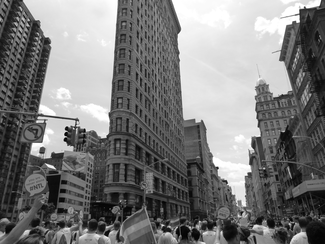
\includegraphics[width=325pt]{pride.png}
Marching in the NYC Pride Parade \\
The Flatiron Building \\
24 June 2012
{\tt kula.tproa.net/photos/2012/2012-pride/ }

\end{center}

\newpage

\thispagestyle{empty}
\vspace*{12cm}
\begin{sideways}
\Large{St. Joshua Norton Press}
\end{sideways}
\begin{sideways}
\Large{PO Box 250138}
\end{sideways}
\begin{sideways}
\Large{New York NY 10025}
\end{sideways}


\end{document}


